%----------------------------------------------------------------------------
%----------------------------------------------------------------------------
%				    	SETUP
%----------------------------------------------------------------------------
%----------------------------------------------------------------------------

\documentclass[12pt]{article}

%----------------------------------------------------------------------------
%			  	   PACKAGES
%----------------------------------------------------------------------------

%% Fonts and Symbols
%% --------------------------
\usepackage[T1]{fontenc}			% better font encoding
\usepackage[utf8]{inputenc}		% better font encoding
%\usepackage[usenames,dvipsnames,svgnames,table]{xcolor}		% allow colour
\usepackage{amsmath,amssymb,amsthm,textcomp, xfrac}		% math symbols, etc
%\usepackage{color}
\usepackage[hidelinks]{hyperref}	% hyperlinks, see config in LAYOUT AND STYLING


%% Graphics
%% --------------------------
\usepackage{graphicx}			% allow insertion of images
\graphicspath{ {./graphics/} }		% the relative path to the graphics folder
%\usepackage{tikz}				% vector graphics
%\usepackage{pgfplots}			% plots in vector graphics


%% Tables
%% --------------------------
\usepackage{booktabs}			% better tables, discourages vertical rulings
%\usepackage{tabularx}
%\usepackage{enumerate}		
\usepackage{multicol}			%allow multi columns


%% Layout Alteration
%% --------------------------
\usepackage{lastpage}
\usepackage{fancyhdr}			% see config in LAYOUT AND STYLING
\usepackage{fullpage}			% set full page margins
%sideways figures
%\usepackage{rotating}
%\usepackage{pdflscape}
%\usepackage{parskip}			% disable indents

%% Units
%% --------------------------
\usepackage{siunitx}			% has S (decimal align) column type
\sisetup{input-symbols = {()},  % do not treat "(" and ")" in any special way
         group-digits  = false} % no grouping of digits
%\sisetup{load-configurations = abbreviations}
%\sisetup{per-mode = symbol}
%\usepackage{cancel}

%% Misc
%% --------------------------
%\usepackage{mhchem}			% chemistry


%----------------------------------------------------------------------------
%		     MACROS AND COMMANDS
%----------------------------------------------------------------------------

%type Y - even column width - centered
% must include tabularx package
%\newcolumntype{Y}{>{\centering\arraybackslash}X}	

% Defines a new command for the horizontal lines, change thickness here
\newcommand{\HRule}{\rule{\linewidth}{0.5mm}} 	

% ???
\newcommand{\linia}{\rule{\linewidth}{0.5pt}}

% scientific notation  use \e
\providecommand{\e}[1]{\ensuremath{\times 10^{#1}}}

% diferential
\def \d {\ensuremath{\mathrm{d}}}

%----------------------------------------------------------------------------
%		   	LAYOUT AND STYLING
%----------------------------------------------------------------------------

% custom footers and headers
% must include fancyhdr package
\pagestyle{fancy}
\lhead{}
\chead{}
\rhead{}
\lfoot{}
\cfoot{\thepage\ of \pageref{LastPage}}
\rfoot{}
\renewcommand{\headrulewidth}{0pt}
\renewcommand{\footrulewidth}{0pt}


%%section style
%\usepackage{titlesec}
%\titleformat{\section}[runin]
%{\normalfont\bfseries}
%{\thesection.}{.5em}{}[]
%
%\titleformat{\subsection}[runin]
%{\normalfont\bfseries}
%{\thesubsection}{.5em}{}[]
%\setcounter{secnumdepth}{0} %dont number sections

%\hypersetup{
%%    	colorlinks=false, 		% set true if you want colored links
%   		linktoc=all,     			% set to all if you want both sections and subsections linked
%%  		linkcolor=blue,  			% choose some color if you want links to stand out
%}


%----------------------------------------------------------------------------
%----------------------------------------------------------------------------
%				   DOCUMENT
%----------------------------------------------------------------------------
%----------------------------------------------------------------------------

\begin{document}

%----------------------------------------------------------------------------
%				    TITLE PAGE
%----------------------------------------------------------------------------

\begin{titlepage}

\center
 
% Header
\textsc{\LARGE University of Victoria}\\[1cm] 	% Name of your university/college
\textsc{\Large ELEC 250}\\[0.5cm] 			% Major heading such as course name
\textsc{\large Linear Circuits I}\\[0.5cm] 		% Minor heading such as course title


% Lab Title
\HRule \\[0.4cm]
{ \huge \bfseries Lab 2 - Phasor Analysis}\\[0.2cm] % Title of your document
\HRule \\[1.5cm]
 
 
%Lab Instructor Details
\begin{minipage}{0.7\textwidth}
\begin{flushleft} 

\large\emph{Instructor:} \\
Dr. Nikitas \textsc{Dimopoulos} \\
\vspace{12 pt}
\emph{Teaching Assistant:} \\
Zhen \textsc{Liu}

\end{flushleft}
\end{minipage}
~
%% No content here, but it keeps the alignment of the instructor/TA
%% box correct.
%% Consider revising.
\begin{minipage}{0.1\textwidth}
\begin{flushright} \large
%Dr. Barbara \textsc{Sawicka} \\
\vspace{12 pt}
%\emph{Teaching Assistant:} \\
%Vahid \textsc{Moradi}
\end{flushright}
\end{minipage}\\[2cm]


% Lab members
\Large Clayton \textsc{Kihn}
\large V00794569	\\
\Large Yves \textsc{Senechal}
\large V00213837	\\
\Large Tyler \textsc{Stephen}
\large V00812021	\\
A01 - B01\\[1.5cm] 


% Date
{\large \today}\\ % Date, change the \today to a set date if you want to be precise

% Logo
\begin{figure}[b]	 % put logo at bottom of the page
	\centering
	\includegraphics[scale=0.3]{UVic_logo}
\end{figure}

\end{titlepage}

%----------------------------------------------------------------------------
%			  TABLE OF CONTENTS
%----------------------------------------------------------------------------

%\tableofcontents
%\pagebreak

%\listoffigures
%\pagebreak

%----------------------------------------------------------------------------
%				    BODY
%----------------------------------------------------------------------------

\section{Object}\label{sec:object}
This lab will study the steady-state responses of an RC and RL circuit when exposed to a purely sinusoidal voltage source. The current response and the phase shift of current relative to voltage will be calculated and compared with measured values.

\section{Results}\label{sec:results}
An Agilent 33220A signal generator was used to create the sinusoidal voltage source used in this lab. A peak-to-peak voltage of 10.5V was used for both circuits. Different frequencies were used in each section and is discussed further in sections \ref{sec:rc} and \ref{sec:rl}.

An Agilent DSOX-2012A oscilloscope was used to analyze the maximal current and phase shift.

\subsection{RC Circuit}\label{sec:rc}
The circuit was connected as show in figure \ref{fig:rc} using selectable capacitor and resistor boxes provided in the lab. A 5 nF capacitor was used in the circuit. A sinusoidal voltage source with a frequency 10 kHz was applied to the circuit.

\begin{figure}[h]
	\centering
	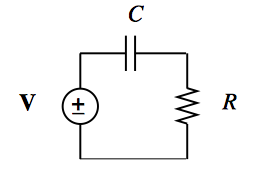
\includegraphics[scale=0.6]{RC_circuit}
	\caption{The RC circuit used in the lab}
	\label{fig:rc}
\end{figure}

The expected phase shift, with current leading voltage, is given by equation \eqref{eqn:rc_theta}, where $\omega = 2\pi f$. The expected maximum current is given by equation \eqref{eqn:rc_current}.

\begin{equation}
	\tan { \theta  } =\left( \frac { 1 }{ \omega RC }  \right) 
	\label{eqn:rc_theta}
\end{equation}

\begin{equation}
		I_{max}(t) = \frac{V_{max}(t)}{\sqrt{R^2 + (\frac{1}{C\omega})^2} }
		\label{eqn:rc_current}
\end{equation}

\pagebreak
The calculated and measured values of the current ($I$) and phase shift ($\theta$) are summarized in table \ref{table:rc}.

\begin{table}[h]
	\centering
	\begin{tabular}{c c c c c}
		\toprule
		&				\multicolumn{2}{c}{Calculated}	& \multicolumn{2}{c}{Measured}	\\
		\cline{2-5}
		$R$ (k$\Omega$)	& $I$ (mA) 	& $\theta$ ($^\circ$) 	& $I$ (mA) 	& $\theta$ ($^\circ$) \\
		\hline
		1				& 3.15		& 72.56					& 3.10			&	70.89	\\
		5				& 1.77		& 32.48					& 1.76			&	31.12	\\
		10				& 1.00		& 17.67					& 0.98			&	14.89	\\
		\toprule
	\end{tabular}
	\caption{Calculated and measured values in the RC circuit}
	\label{table:rc}
\end{table}

\subsection{RL Circuit}\label{sec:rl}
The circuit was connected as shown in figure \ref{fig:rl}. The resistor box was reused and discrete inductors were obtained from the lab (see tables \ref{table:rl_calc} and \ref{table:rl_meas}). The frequency of the voltage source was set to 500 kHz.

\begin{figure}[h]
	\centering
	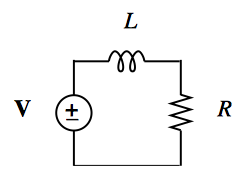
\includegraphics[scale=0.6]{RL_circuit}
	\caption{The RL circuit used in the lab}
	\label{fig:rl}
\end{figure}

The expected phase shift of current with respect to voltage is given by equation \eqref{eqn:rl_theta}. The negative sign indicates that voltage will lead current. The expected maximum current is given by equation \eqref{eqn:rl_current}.

\begin{equation}
	\tan { \theta  } =\left( \frac { -\omega L }{ R }  \right) 
	\label{eqn:rl_theta}
\end{equation}

\begin{equation}
		I_{max}(t) = \frac{V_{max}(t)}{\sqrt{R^2 + L^2\omega^2}}
		\label{eqn:rl_current}
\end{equation}

\pagebreak
Calculated values for each pairing of resistor and inductor is summarized in table \ref{table:rl_calc}. Measured results are presented in table \ref{table:rl_meas}.

\begin{table}[h]
	\centering
	\begin{tabular}{c S S S S S S S S}
		\toprule
		& \multicolumn{2}{c}{$1 \mu$H}	& \multicolumn{2}{c}{$220 \mu$H} & \multicolumn{2}{c}{$470 \mu$H} & \multicolumn{2}{c}{$1000 \mu$H} \\
		\cline{2-9}
		$R$ (k$\Omega$)	& \multicolumn{1}{c}{$I$ (mA)} 	& \multicolumn{1}{c}{$\theta$ ($^\circ$)} 	& \multicolumn{1}{c}{$I$ (mA)} 	& \multicolumn{1}{c}{$\theta$ ($^\circ$)}	& \multicolumn{1}{c}{$I$ (mA)} 	& \multicolumn{1}{c}{$\theta$ ($^\circ$)}	& \multicolumn{1}{c}{$I$ (mA)} 	& \multicolumn{1}{c}{$\theta$ ($^\circ$)} \\
		\hline
		1		& 10.50	& -0.18	& 8.64	& -34.65& 5.89	& -55.89& 3.18	& -72.34\\
		5		& 2.10	& -0.04	& 2.08	& -7.87	& 2.01	& -16.45& 1.78	& -32.14\\
		10		& 1.05	& -0.02	& 1.05	& -3.95	& 1.04	& -8.40	& 1.00	& -17.44\\
		\toprule
	\end{tabular}
	\caption{Calculated values in the RL circuit}
	\label{table:rl_calc}
\end{table}

\begin{table}[h]
	\centering
	\begin{tabular}{c S S S S S S S S}
		\toprule
		& \multicolumn{2}{c}{$1 \mu$H}	& \multicolumn{2}{c}{$220 \mu$H} & \multicolumn{2}{c}{$470 \mu$H} & \multicolumn{2}{c}{$1000 \mu$H} \\
		\cline{2-9}
		$R$ (k$\Omega$)	& \multicolumn{1}{c}{$I$ (mA)} 	& \multicolumn{1}{c}{$\theta$ ($^\circ$)} 	& \multicolumn{1}{c}{$I$ (mA)} 	& \multicolumn{1}{c}{$\theta$ ($^\circ$)}	& \multicolumn{1}{c}{$I$ (mA)} 	& \multicolumn{1}{c}{$\theta$ ($^\circ$)}	& \multicolumn{1}{c}{$I$ (mA)} 	& \multicolumn{1}{c}{$\theta$ ($^\circ$)} \\
		\hline
		1	& 3.00	& -84	& 9.00	& -36	& 6.00	& -63	& 3.18	& -82 \\
		5	& 2.46	& -61	& 2.34	& -9	& 2.58	& -25	& 2.66	& -58 \\
		10	& 2.01	& -51	& 1.17	& -5	& 1.41	& -13	& 2.01	& -42 \\
		\toprule
	\end{tabular}
	\caption{Measured values in the RL circuit}
	\label{table:rl_meas}
\end{table}


\section{Discussion and Conclusion}\label{sec:d_and_c}
The RC series circuit performed as expected. Minor discrepancies in phase shift and circuit current were observed which could be attributed to the use of non-ideal components that introduce a factor of uncertainty. 

The RL series circuit performed nearly as expected for the $220\mu H$ with the $470\mu H$ and $1mH$ varying slightly. The discrepancies between measured and calculated values could be attributed to: \textit{(a)heat:} results in added resistance produced by the components, and \textit{(b)use of non-ideal components:} each circuit component adds a degree of uncertainty. 

The $1\mu H$ inductor circuit, whether combined with the $1k\Omega$, $5k\Omega$, or the $10k\Omega$ resistors, provided results that appeared nearest to the values expected of a $1m H$. This part of the experiment was performed with two different inductors that yielded similar results. Possible justification for these discrepancies include: \textit{(a)faulty components:} in this case, both $1\mu H$ inductors must be faulty, or \textit{(b)mislabeled inductors:} the difference between the symbol for $mH$ and $\mu H$ may be difficult to differentiate when handwritten on heat shrink.

Capacitors are more predictable than inductors when connected to a circuit. This could be due to a by-product of heat produced within an inductor, or the improved accuracy of mass-producing capacitors versus inductors.



%----------------------------------------------------------------------------
%				  LaTeX TIPS
%----------------------------------------------------------------------------

\pagebreak

\section{LaTeX Tips}\label{sec:tips}
Check the source file for additional information in the comments.
\subsection{Symbols}\label{sec:symbols}
Most math symbols and all equations are bounded by \$ delimiters. \verb|$ A=\pi r^{2} $| produces $ A=\pi r^{2} $. To find the appropriate symbol you will have to use a LaTeX IDE with a built in symbol editor or use another program to produce the code and copy-and-paste it into your document.

\subsection{Figures}\label{sec:figures}
\begin{verbatim}
\begin{figure}[h]
	\centering
	\includegraphics[width=0.75\textwidth]{Uvic_logo}
	\caption{A logo used by the University of Victoria}
	\label{fig:uvic_logo}
\end{figure}
\end{verbatim}

\begin{figure}[h] 	% placement in document [htbp]: here, top, bottom, special page
	\centering		% centers the image
	\includegraphics[width=0.75\textwidth]{Uvic_logo} 	
		% will search root directory and anything listed
		% in \graphicspath for the image
		% it is common to specify [width=0.5\textwidth] as an agument
		% \textwidth can be used as a variable for the entire pagewidth.
		% 0.5\textwidth refers to 50% of the page.
	\caption{A logo used by the University of Victoria}
	\label{fig:uvic_logo}
\end{figure}

A good tutorial for the use of figures can be found at: \url{http://en.wikibooks.org/wiki/LaTeX/Floats,_Figures_and_Captions}

\pagebreak
\subsection{Tables}\label{sec:tables}
\begin{verbatim}
\begin{table}[h]
	\centering
	\begin{tabular}{llr}
		\hline
		\multicolumn{2}{c}{Item} \\
		\cline{1-2}
			Animal   	& Description 	& Price (\$) \\
		\hline
			Gnat		& per gram	& 13.65      \\
				        & each       	& 0.01       \\
			Gnu		& stuffed     	& 92.50      \\
			Emu		& stuffed		& 33.33      \\
			Armadillo	& frozen		& 8.99       \\
		\hline
	\end{tabular}
	\caption{Exotic meat prices}
	\label{table:meats}
\end{table}
\end{verbatim}

\begin{table}[h]			% placement in document [htbp]: [h]ere, [t]op, [b]ottom, special [p]age
	\centering
	\begin{tabular}{llr}	% specifies the number of columns and their justification
					% columns can be [l]eft-justified, [c]entered, [r]ight-justified
					% the number of arguments after {tabular} corresponds to the number of columns
					% vertical lines can be added by placing | vertical bars in the argument
					% e.g. { | c c c | } has three centered columns with vertical lines at the ends
					% of the table
					% { | c | c | c | } has vertical lines separating all cells

		\hline		% a horizontal line
		
		\multicolumn{2}{c}{Item} \\		% {number of columns to span}{lcr}{title}
								% \\ indicates the end of a line
								
		\cline{1-2}		% \cline[ i - j } : line that spans columns i to j
		
			Animal   	& Description 	& Price (\$) \\	% & separates data between cells
											% && indicates a blank cell
											% \\ must end every row
		\hline
			Gnat		& per gram		& 13.65      \\
				    	& each      	 	& 0.01       \\
			Gnu		& stuffed     	& 92.50      \\
			Emu		& stuffed		& 33.33      \\
			Armadillo	& frozen		& 8.99       \\
		\hline
	\end{tabular}
	\caption{Exotic meat prices}
	\label{table:meats}
\end{table}
\textit{Apparently} tables are more readable if the vertical rulings are omitted. I'm inclined to agree.\\
A good tutorial for the use of tables can be found at: \url{http://en.wikibooks.org/wiki/LaTeX/Tables}

\subsection{Labels and References}\label{sec:labels_and_refs}
LaTeX's dynamic referencing system gives it an advantage over other multi-user document tools. References point to assigned labels rather than a pre-defined numbering. Changing the order and number of references will leave the citations untouched if label referencing is used.


The \verb|\label{}| tag should be attached to all sections, figures and tables. To reference these elements, use the \verb|\ref{}| command. To reference the table in Section \ref{sec:tables}, you would write \verb|Table \ref{table:meats}| which will appear as Table \ref{table:meats}.


A consistent naming schema will make collaboration easier. Labels should be implemented with the corresponding prefix:
\begin{table}[h]
	\centering
	\begin{tabular}{ l l }
	Sections		& \verb|{sec:}|		\\
	Figures		& \verb|{fig:}|		\\
	Tables		& \verb|{table:}|		\\
	\end{tabular}
\end{table}

You may encounter a situation where a citation or page number appears as \verb|??|. This often occurs when major changes have occured to the reference or page order. The LaTeX compiler requires two executions of the typesetting function to correctly address the references: one to build the .aux file and another to read from it. The compiler is often nice enouch to pass a warning when the .aux file has undergone significant changes to its references and prompts you do another typesetting.

\subsection{Resources}\label{sec:resources}
\begin{itemize}
	\item \underline{\href{https://www.youtube.com/user/14mech14/videos}{Video playlist} } from McMaster that covers the installation and use of LaTeX. Uses TeXShop for examples. Covers document setup, tables, figures, bibliographies and some other stuff I haven't watched yet.
\end{itemize}

%----------------------------------------------------------------------------
%----------------------------------------------------------------------------
%			DO NOT DELETE BELOW
%----------------------------------------------------------------------------
%----------------------------------------------------------------------------

\end{document}